En esta sección el objetivo será comparar todos los algoritmos diseñados e implementados en este trabajo.

A continuación incluiremos dos gráficos. Uno para poder observar como se comportan tanto nuestros algoritmos ante la familia de grafos \emph{3-caminos} y otro ante la familia \emph{3-caminos con puentes}.

\begin{figure}[H]
    \begin{minipage}{0.5\linewidth}
      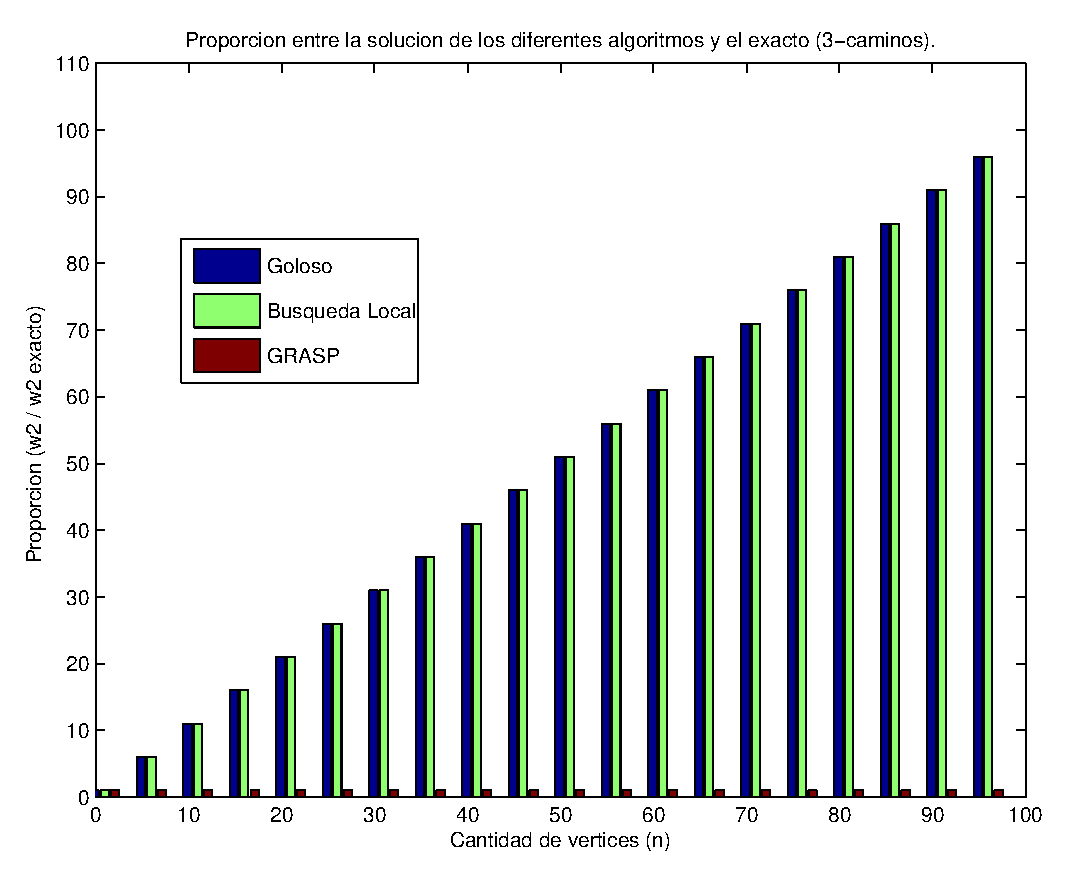
\includegraphics[width=\linewidth]{graficos/todos_proporcion_3caminos.eps}
      \caption{Comportamiento ante familia \emph{3-caminos}}\label{fig:comportamiento-familia-rompe}
    \end{minipage}
    \hfill
    \begin{minipage}{0.5\linewidth}
      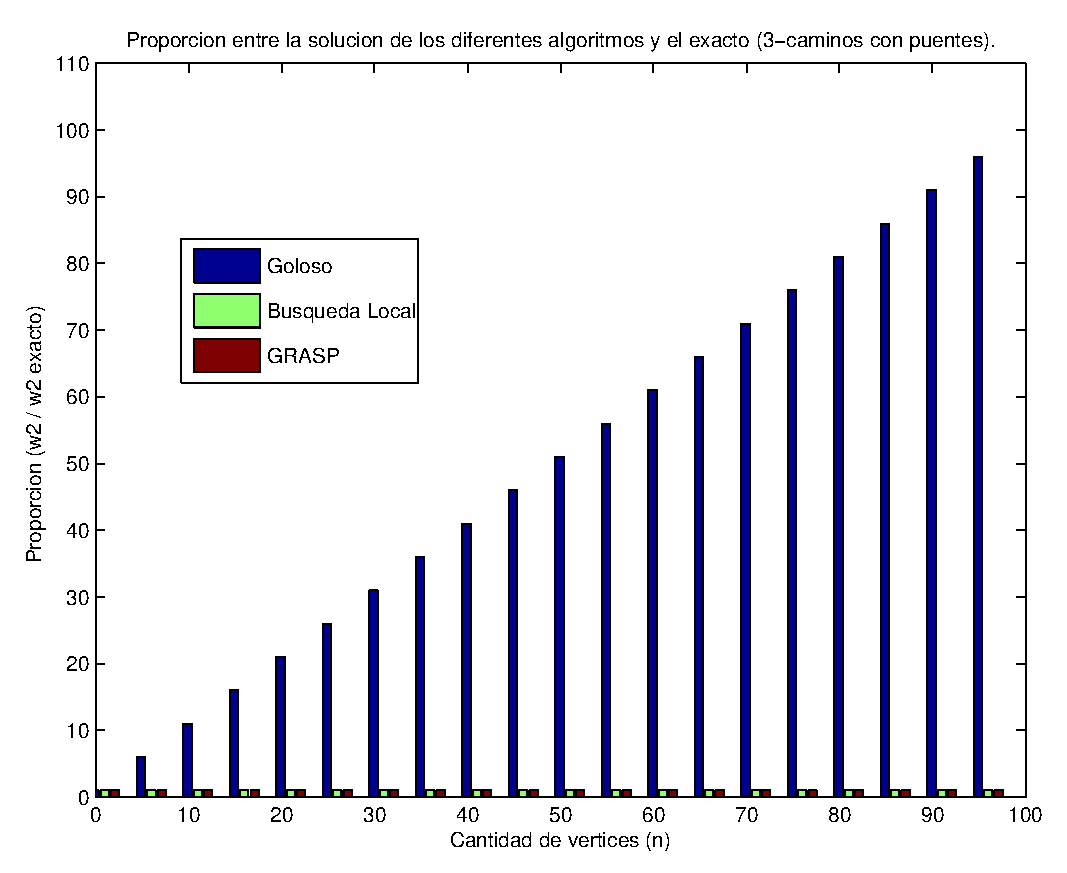
\includegraphics[width=\linewidth]{graficos/todos_proporcion_puentes.eps}
      \caption{Ídem familia \emph{3-caminos con puentes}}\label{fig:comportamiento-familia-puente}
    \end{minipage}    
\end{figure}

En estos gráficos mostramos el comportamiento de tanto de los siguientes algoritmos para dos familias de grafos. Los algoritmos medidos son los siguientes (todos en proporción al algoritmo exacto):

\begin{itemize}
 \item Algoritmo Goloso implementado en el trabajo.
 \item Algoritmo de búsqueda local, que utiliza nuestro algoritmo goloso.
 \item Algoritmo GRASP que utiliza nuestro algoritmo goloso aleatorio y nuestro algoritmo de búsqueda local.
\end{itemize}

Vale aclarar que todas las soluciones se muestran en proporción a las del algoritmo exacto.

En el gráfico de la Figura \ref{fig:comportamiento-familia-rompe} podemos ver que para los grafos de la familia \emph{3-caminos} nuestro algoritmo goloso devuelve soluciones de mala calidad, al igual que nuestro algoritmo de búsqueda local. Sin embargo, nuestro algoritmo GRASP logra mejorar las soluciones de dichos algoritmos. Más aún, no solo las mejora sino que devuelve la solución óptima. También podemos volver a ver que nuestro algoritmo de búsqueda local no logra mejorar la solución inicial que le da el algoritmo goloso para esta familia de grafos cuando éstos superan una determinada cantidad de nodos (en secciones previas observamos que dicha cantidad es $7$).

A su vez, en el gráfico de la Figura \ref{fig:comportamiento-familia-puente} podemos observar que nuestro algoritmo goloso devuelve malas soluciones para la familia de grafos \emph{3-caminos con puentes}, pero que el algoritmo de búsqueda local las logra mejorar, devolviendo una solución óptima. También podemos ver que el algoritmo GRASP también se comporta de manera óptima para los algoritmos de dicha familia.

Para continuar incluimos un gráfico que compara las soluciones de nuestro algoritmo GRASP y nuestro algoritmo de búsqueda local en proporción con nuestro algoritmo goloso.

\begin{figure}[H]
  \begin{center}
    \begin{minipage}{0.5\linewidth}
    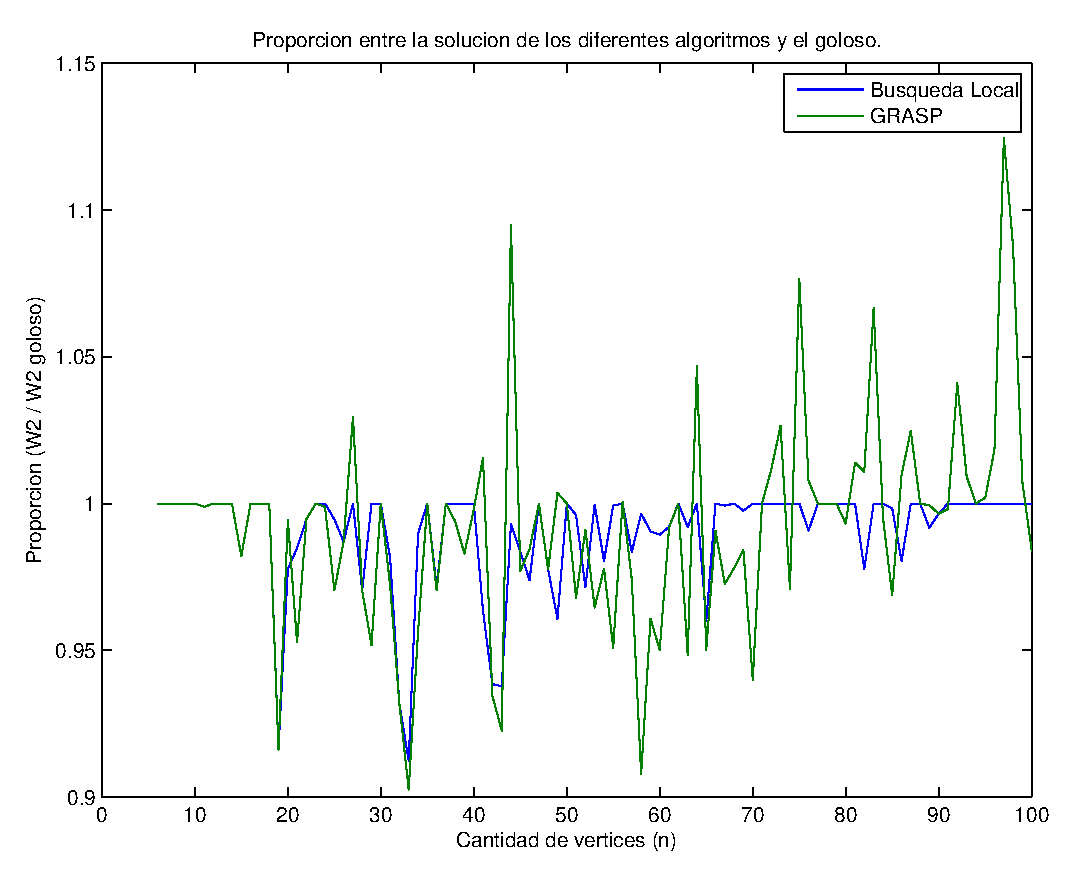
\includegraphics[width=\linewidth]{graficos/todos_calidad.eps}
    \caption{Soluciones en proporción con goloso}\label{fig:proporcion-goloso}
    \end{minipage}
  \end{center}
\end{figure}

El algoritmo de búsqueda local siempre da soluciones que son mejores o iguales a las que da el algoritmo goloso, ya que la proporción es siempre menor o igual a uno. Esto es lógico ya que nuestro algoritmo de búsqueda local toma como solución inicial la que da el goloso e intenta mejorarlas, lo cual no siempre logra, pero nunca empeora la solución inicial que se le da.

Además, podemos ver que las soluciones que da el algoritmo GRASP son a veces mejores que las del algoritmo de búsqueda local pero a veces son peores. Esto es debido a que el algoritmo de GRASP hace búsqueda local sobre la solución inicial que le da nuestro algoritmo goloso aleatorio en cada iteración. Por lo tanto, GRASP hace búsqueda local a partir de soluciones iniciales distintas a la del algoritmo de búsqueda local que toma como solución inicial la dada por nuestro algoritmo goloso que no es aleatorio. Entonces, tiene sentido que GRASP llegue a soluciones distintas al algoritmo de búsqueda local, las cuales a veces son mejores y a veces son peores.
